\subsection{Scenario Richieste}
\begin{figure}[H] 
    \centering 
    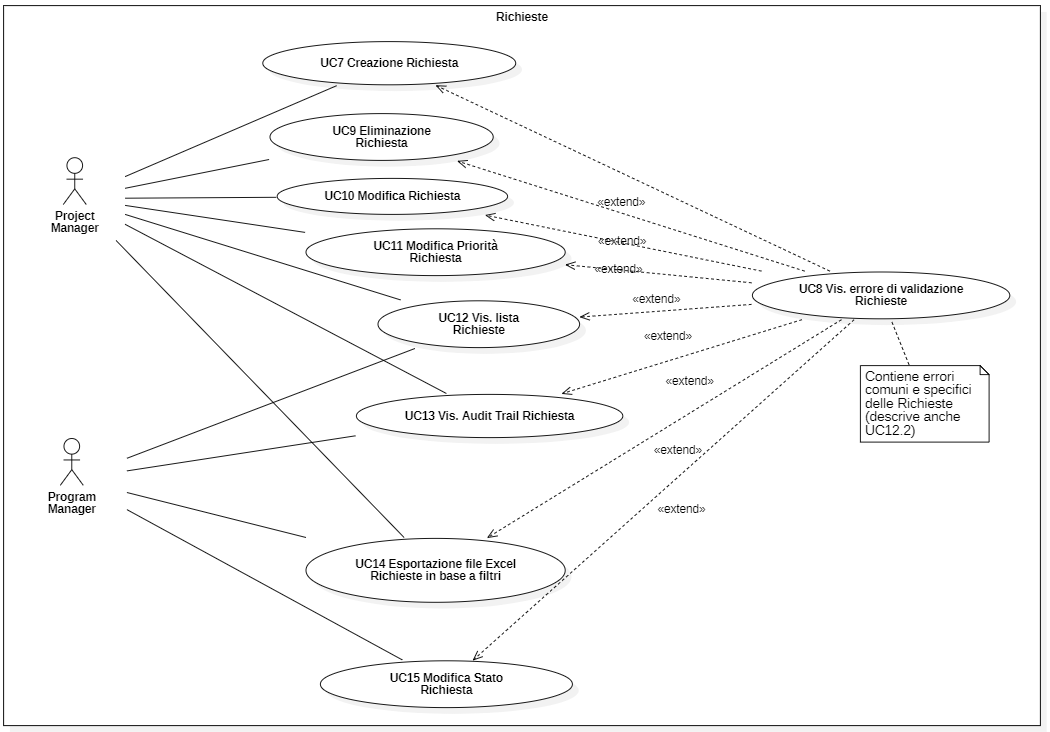
\includegraphics[width=1.15\columnwidth]{usecase/richieste-general} 
    \caption{Casi d'Uso del scenario Richieste}
\end{figure}

\subsubsection*{UC7 - Creazione Richiesta}
\begin{itemize}[label=$\circ$]
\item \textbf{Attore:} Project Manager;
\item \textbf{Descrizione:} il Project Manager può creare una nuova Richiesta;
\item \textbf{Precondizioni:} il richiedente è un Project Manager;
\item \textbf{Postcondizioni:} la Richiesta è stata creata dal Project Manager con successo;
\item \textbf{Estensioni:} UC8;
\item \textbf{Inclusioni:} il caso d'uso non ha inclusioni.
\end{itemize}

\subsubsection*{UC8 - Vis. errore di validazione Richieste}
\begin{itemize}[label=$\circ$]
\item \textbf{Attore:} Project Manager e Program Manager;
\item \textbf{Descrizione:}  questo caso d'uso descrive anche UC12.2. Viene visualizzato un messaggio di errore in caso vengano eseguite funzionalità con dati non validi. Esso rappresenta i seguenti errori comuni all'interno delle Richieste: dati non validi, filtri non valorizzati, entità associate non valide, risultati nulli o non valorizzati;
\item \textbf{Precondizioni:} il Program Manager o il Project Manager stanno effettuando operazioni con dati non validi;
\item \textbf{Postcondizioni:} l'esecuzione della funzionalità è interrotta e viene visualizzato il messaggio di errore;
\item \textbf{Estensioni:} il caso d'uso non ha estensioni;
\item \textbf{Inclusioni:} il caso d'uso non ha inclusioni.
\end{itemize}

\subsubsection*{UC9 - Eliminazione Richiesta}
\begin{itemize}[label=$\circ$]
\item \textbf{Attore:} Project Manager;
\item \textbf{Descrizione:} il Project Manager può eliminare una Richiesta esistente;
\item \textbf{Precondizioni:} il richiedente è un Project Manager;
\item \textbf{Postcondizioni:} la Richiesta è stata eliminata dal Project Manager con successo;
\item \textbf{Estensioni:} UC8;
\item \textbf{Inclusioni:} il caso d'uso non ha inclusioni.
\end{itemize}

\subsubsection*{UC10 - Modifica Richiesta}
\begin{itemize}[label=$\circ$]
\item \textbf{Attore:} Project Manager;
\item \textbf{Descrizione:} il Project Manager può modificare una Richiesta esistente nella sua totalità sovrascrivendola;
\item \textbf{Precondizioni:} il richiedente è un Project Manager;
\item \textbf{Postcondizioni:} la Richiesta selezionata è stata modificata con successo;
\item \textbf{Estensioni:} UC8;
\item \textbf{Inclusioni:} il caso d'uso non ha inclusioni.
\end{itemize}

\subsubsection*{UC11 - Modifica Priorità Richiesta}
\begin{itemize}[label=$\circ$]
\item \textbf{Attore:} Project Manager;
\item \textbf{Descrizione:} il Project Manager può modificare l'attributo Priorità di una Richiesta esistente inserendo un valore tra: Alta, Media o Bassa;
\item \textbf{Precondizioni:} il richiedente è un Project Manager;
\item \textbf{Postcondizioni:} la Richiesta è stata modificata con successo solo nel campo Priorità dal Project Manager;
\item \textbf{Estensioni:} UC8;
\item \textbf{Inclusioni:} il caso d'uso non ha inclusioni.
\end{itemize}

\subsubsection*{UC12 - Vis. lista Richieste}

\begin{figure}[H] 
    \centering 
    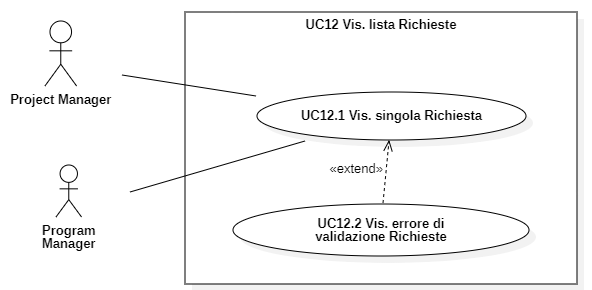
\includegraphics[width=0.7\columnwidth]{usecase/UC12} 
    \caption{Caso d'Uso 12 espanso}
\end{figure}

\begin{itemize}[label=$\circ$]
\item \textbf{Attore:} Project Manager e Program Manager;
\item \textbf{Descrizione:} il Project Manager e il Program Manager possono visualizzare una lista di Richieste dopo aver inserito filtri e/o una parola nella ricerca rapida e aver selezionato se i filtri applicati devono essere congiunti o disgiunti;
\item \textbf{Precondizioni:} il richiedente è un Project Manager o un Program Manager;
\item \textbf{Postcondizioni:} la lista delle Richieste è visualizzabile dal Project Manager e dal Program Manager;
\item \textbf{Estensioni:} UC8;
\item \textbf{Inclusioni:} il caso d'uso non ha inclusioni.
\end{itemize}

\subsubsection*{UC12.1 - Vis. singola Richiesta}

\begin{figure}[H] 
    \centering 
    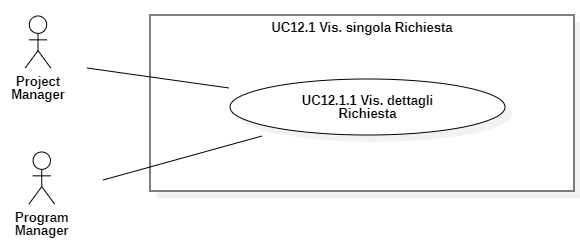
\includegraphics[width=0.7\columnwidth]{usecase/UC12.1} 
    \caption{Caso d'Uso 12.1 espanso}
\end{figure}

\begin{itemize}[label=$\circ$]
\item \textbf{Attore:} Project Manager e Program Manager;
\item \textbf{Descrizione:} il Project Manager e il Program Manager possono visualizzare la Richiesta selezionata;
\item \textbf{Precondizioni:} la lista delle Richieste è visualizzabile;
\item \textbf{Postcondizioni:} la Richiesta selezionata è visualizzabile dal Program Manager e dal Project Manager;
\item \textbf{Estensioni:} UC12.2;
\item \textbf{Inclusioni:} il caso d'uso non ha inclusioni.
\end{itemize}

\subsubsection*{UC12.1.1 - Vis. dettagli Richiesta}

\begin{itemize}[label=$\circ$]
\item \textbf{Attore:} Project Manager e Program Manager;
\item \textbf{Descrizione:} il Project Manager e il Program Manager possono visualizzare la Richiesta selezionata;
\item \textbf{Precondizioni:} la Richiesta singola è visualizzabile;
\item \textbf{Postcondizioni:} il Project Manager e il Program Manager possono visualizzare i campi di una Richiesta selezionata;
\item \textbf{Estensioni:} il caso d'uso non ha esclusioni;
\item \textbf{Inclusioni:} il caso d'uso non ha inclusioni.
\end{itemize}

\subsubsection*{UC13 - Vis. audit\textsubscript{g} trail Richiesta}

\begin{figure}[H] 
    \centering 
    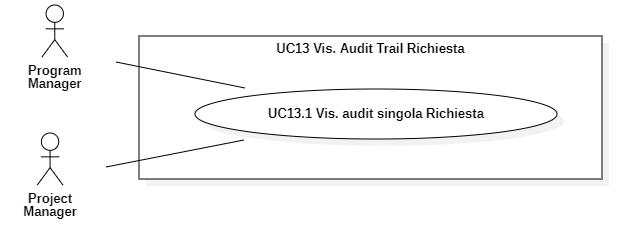
\includegraphics[width=0.7\columnwidth]{usecase/UC13} 
    \caption{Caso d'Uso 13 espanso}
\end{figure}

\begin{itemize}[label=$\circ$]
\item \textbf{Attore:} Project Manager e Program Manager;
\item \textbf{Descrizione:} il Project Manager e il Program Manager possono visualizzare l'audit trail di una Richiesta selezionata.;
\item \textbf{Precondizioni:} il richiedente è un Project Manager o un Program Manager;
\item \textbf{Postcondizioni:} la traccia di audit della Richiesta selezionata è visualizzabile dal Project Manager e dal Program Manager;
\item \textbf{Estensioni:} UC8;
\item \textbf{Inclusioni:} il caso d'uso non ha inclusioni.
\end{itemize}

\subsubsection*{UC13.1 - Vis. audit singola Richiesta}

\begin{figure}[H] 
    \centering 
    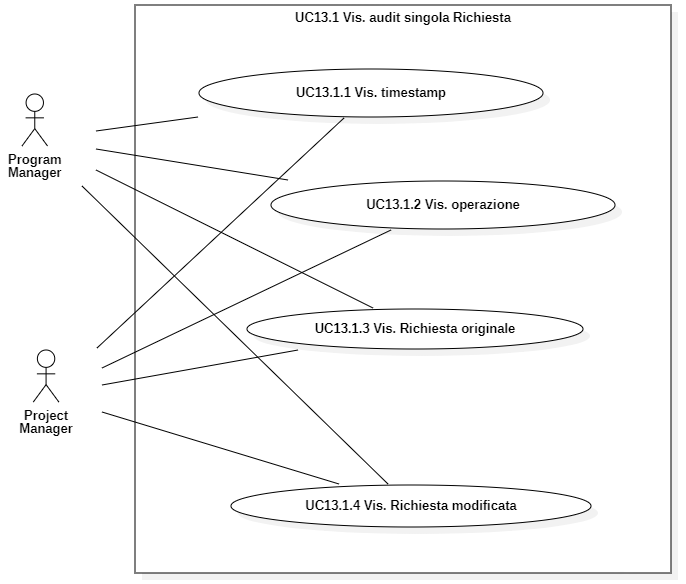
\includegraphics[width=0.8\columnwidth]{usecase/UC13.1} 
    \caption{Caso d'Uso 13.1 espanso}
\end{figure}

\begin{itemize}[label=$\circ$]
\item \textbf{Attore:} Project Manager e Program Manager;
\item \textbf{Descrizione:} il Project Manager e il Program Manager possono visualizzare l'audit di una singola Richiesta;
\item \textbf{Precondizioni:} l'audit trail è visualizzabile;
\item \textbf{Postcondizioni:} l'audit di una singola Richiesta è visualizzabile;
\item \textbf{Estensioni:} il caso d'uso non ha estensioni;
\item \textbf{Inclusioni:} il caso d'uso non ha inclusioni.
\end{itemize}

\subsubsection*{UC13.1.1 - Vis. timestamp\textsubscript{g}}
\begin{itemize}[label=$\circ$]
\item \textbf{Attore:} Project Manager e Program Manager;
\item \textbf{Descrizione:} il Project Manager e il Program Manager possono visualizzare il timestamp di una singola audit di una Richiesta;
\item \textbf{Precondizioni:} la singola audit di una Richiesta è visualizzabile;
\item \textbf{Postcondizioni:} il timestamp della singola audit è visualizzabile;
\item \textbf{Estensioni:} il caso d'uso non ha estensioni;
\item \textbf{Inclusioni:} il caso d'uso non ha inclusioni.
\end{itemize}

\subsubsection*{UC13.1.2 - Vis. operazione}
\begin{itemize}[label=$\circ$]
\item \textbf{Attore:} Project Manager e Program Manager;
\item \textbf{Descrizione:} il Project Manager e il Program Manager possono visualizzare l'operazione di una singola audit di una Richiesta;
\item \textbf{Precondizioni:} la singola audit di una Richiesta è visualizzabile;
\item \textbf{Postcondizioni:} l'operazione della singola audit è visualizzabile;
\item \textbf{Estensioni:} il caso d'uso non ha estensioni;
\item \textbf{Inclusioni:} il caso d'uso non ha inclusioni.
\end{itemize}

\subsubsection*{UC13.1.3 - Vis. Richiesta originale}
\begin{itemize}[label=$\circ$]
\item \textbf{Attore:} Project Manager e Program Manager;
\item \textbf{Descrizione:} il Project Manager e il Program Manager possono visualizzare la singola audit di una Richiesta prima che l'operazione venga eseguita;
\item \textbf{Precondizioni:} la singola audit di una Richiesta è visualizzabile;
\item \textbf{Postcondizioni:} la Richiesta originale della singola audit è visualizzabile;
\item \textbf{Estensioni:} il caso d'uso non ha estensioni;
\item \textbf{Inclusioni:} il caso d'uso non ha inclusioni.
\end{itemize}

\subsubsection*{UC13.1.4 - Vis. Richiesta modificata}
\begin{itemize}[label=$\circ$]
\item \textbf{Attore:} Project Manager e Program Manager;
\item \textbf{Descrizione:} il Project Manager e il Program Manager possono visualizzare la singola audit di una Richiesta dopo che l'operazione è stata eseguita;
\item \textbf{Precondizioni:} la singola audit di una Richiesta è visualizzabile;
\item \textbf{Postcondizioni:} la Richiesta modificata della singola audit è visualizzabile;
\item \textbf{Estensioni:} il caso d'uso non ha estensioni;
\item \textbf{Inclusioni:} il caso d'uso non ha inclusioni.
\end{itemize}

\subsubsection*{UC14 - Esportazione file Excel Richieste in base a filtri}
\begin{itemize}[label=$\circ$]
\item \textbf{Attore:} Project Manager e Program Manager;
\item \textbf{Descrizione:} il Project Manager e il Program Manager possono esportare in un file Excel scaricabile un report delle Richieste in base a dei filtri inseriti;
\item \textbf{Precondizioni:} il richiedente è un Project Manager o un Program Manager;
\item \textbf{Postcondizioni:} il report Excel è stato generato correttamente ed è possibile scaricarlo;
\item \textbf{Estensioni:} UC8;
\item \textbf{Inclusioni:} il caso d'uso non ha inclusioni.
\end{itemize}

\subsubsection*{UC15 - Modifica Stato Richiesta}
\begin{itemize}[label=$\circ$]
\item \textbf{Attore:} Program Manager;
\item \textbf{Descrizione:} il Program Manager può cambiare lo stato di una Richiesta esistente impostandolo in uno dei seguenti valori: Evasa, Non Evasa, Aperta, In corso, Chiusa;
\item \textbf{Precondizioni:} il richiedente è un Program Manager;
\item \textbf{Postcondizioni:} solo lo stato della Richiesta è stato modificato con successo;
\item \textbf{Estensioni:} UC8;
\item \textbf{Inclusioni:} il caso d'uso non ha inclusioni.
\end{itemize}

